%pre-001
\begin{prerequis}[Prérequis]    
    \begin{itemize}
        \item \ldots
        \item \ldots
        \item \ldots
        \item \ldots
    \end{itemize}
\end{prerequis}


% \hspace{1cm}

% \begin{center}
%     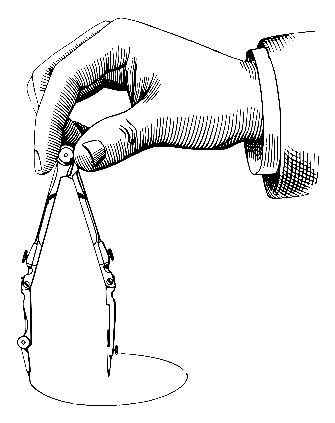
\includegraphics[scale=1]{\currentpath/images/compas.eps}
% \end{center}

\hspace{1cm}

\begin{center}
    \begin{myBox}{La légende de Thalès feat. Arnaud Durand}
        Se munir de papier et d'un crayon et prendre des notes pour pouvoir reparler de ce qui vous aura sembler important.

        \bigskip
        
        \href{http://lozano.maths.free.fr/videos/la-legende-de-thales.mp4}{\emoji{movie-camera} Lancer la vidéo.}
    \end{myBox}

    \begin{myBox}{Petit conte mathématique}
        Se munir de papier et d'un crayon et prendre des notes pour pouvoir reparler de ce qui vous aura sembler important.

        \bigskip
        
        \href{http://lozano.maths.free.fr/videos/TheoremeThales.mp4}{\emoji{movie-camera} Lancer la vidéo france TV.}
    \end{myBox}
\end{center}

\hspace{1cm}

\begin{center}
    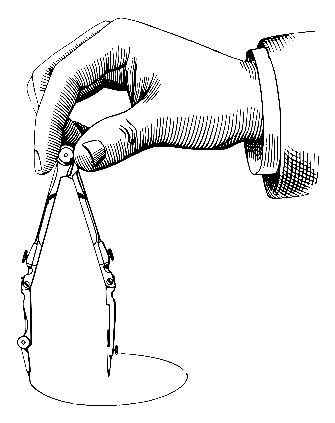
\includegraphics[scale=0.7]{\currentpath/images/compas.eps}
\end{center}

% \vspace{0.9em}
% \begin{autoeval}
%     Nada
% \begin{multicols}{2}
% %000
% \begin{exercice*}
    \ldots
    \begin{ChoixQCM}{4}
        \item \ldots
        \item \ldots
        \item \ldots
        \item \ldots
    \end{ChoixQCM}
\end{exercice*}
\begin{corrige}
    Réponse \reponseQCM{c}, \ldots
\end{corrige}
% \end{multicols}
% \end{autoeval}